\documentclass[tikz]{standalone}
\usepackage{tikz}
\usepackage[AutoFakeBold=true,AutoFakeSlant=true]{xeCJK}
\usepackage[zihao=-4,UTF8,heading=true]{ctex}
\usepackage[simplified]{pgf-umlcd}
\usetikzlibrary{fit} %形状
\usetikzlibrary{positioning} %不加方向运算可能出错
\usetikzlibrary{arrows.meta} %箭头
\usetikzlibrary{calc}

\setCJKmainfont{微软雅黑}
\begin{document}
	\thispagestyle{empty}
    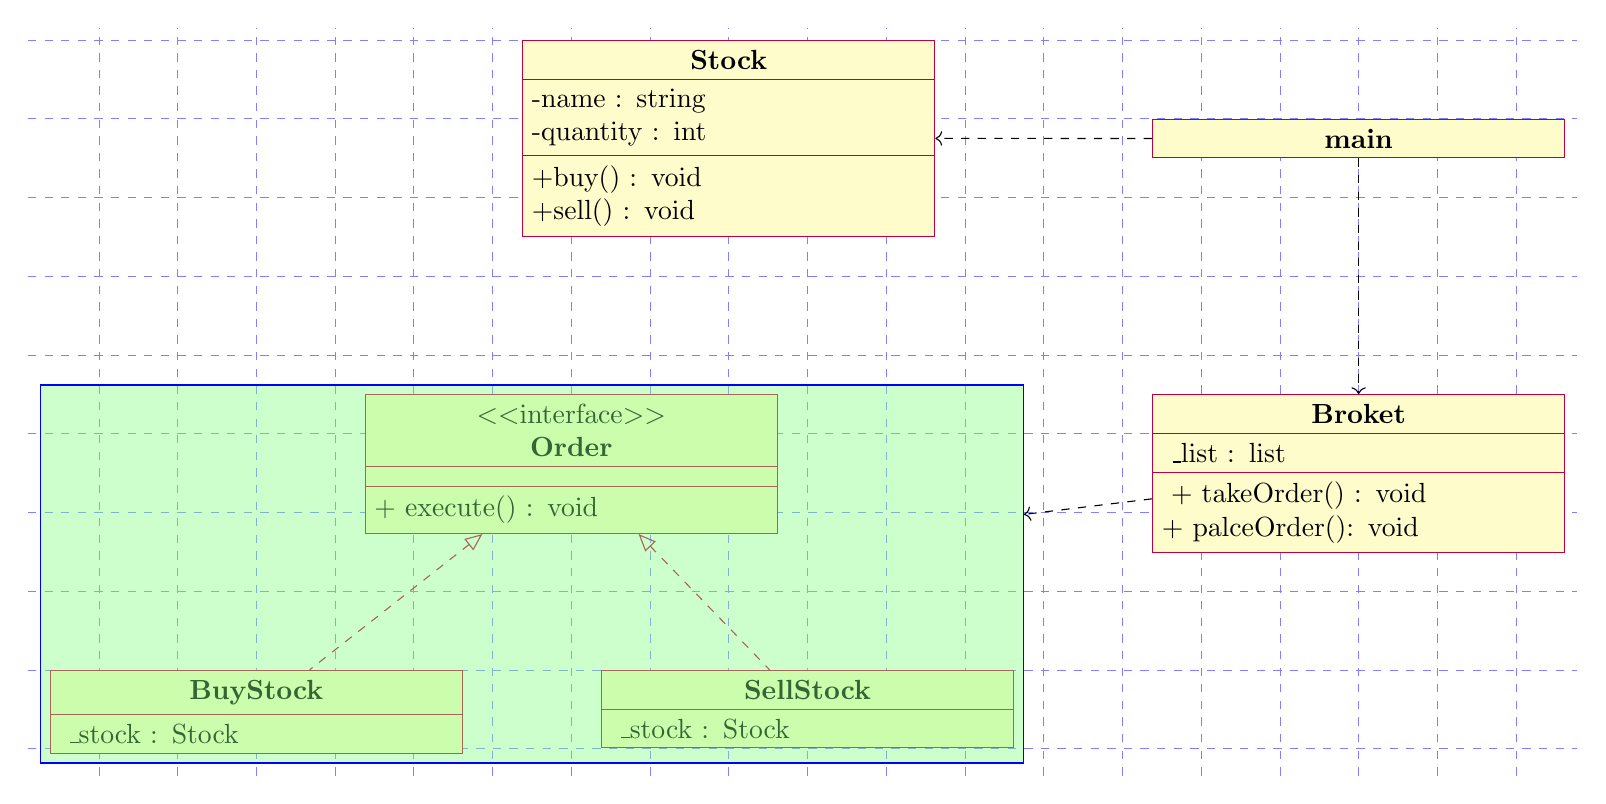
\begin{tikzpicture}[show background grid]
        \begin{class}[text width=5cm]{Stock}{0,0}
            \attribute{-name : string}
            \attribute{-quantity : int }
            \operation{+buy() : void}
            \operation{+sell() : void}
        \end{class}
        
        \begin{interface}[]{Order}{-2, -4.5}
            \attribute{    }
            \operation{+ execute() : void}
        \end{interface}
        \begin{class}[]{BuyStock}{-6,-8}
            \attribute{ \_stock : Stock }
            \implement{Order}
        \end{class}

        \begin{class}[]{SellStock}{1, -8}
             \attribute{ \_stock  : Stock }
             \implement{Order}
        \end{class}
        \node[fill=green!50,fill opacity=.4,
            fit=(Order)(BuyStock)(SellStock),
            draw=blue](OrderSet){};
        \begin{class}[]{Broket}{8,-4.5}
            \attribute{ \_list  : list }
            \operation{ + takeOrder() : void}
            \operation{ + palceOrder(): void}
        \end{class}
        \begin{class}[]{main}{8,-1}
        \end{class}
        
        \draw [dashed, ->] (main) -- (Broket);
        \draw [dashed, ->] (main) -- (Stock);
        \draw [dashed, ->] (Broket) -- (OrderSet);
        
    \end{tikzpicture}
\end{document}